\documentclass[conference]{IEEEtran}
\IEEEoverridecommandlockouts
\usepackage{cite}
\usepackage{amsmath,amssymb,amsfonts}
\usepackage{algorithmic}
\usepackage{graphicx}
\usepackage{textcomp}
\usepackage{xcolor}
\usepackage{tikz}
\usepackage{enumitem}
\setlist[itemize]{topsep=2pt, itemsep=1pt, parsep=0pt}
\usetikzlibrary{arrows.meta,positioning}
\def\BibTeX{{\rm B\kern-.05em{\sc i\kern-.025em b}\kern-.08em
    T\kern-.1667em\lower.7ex\hbox{E}\kern-.125emX}}

\begin{document}

\title{Visualec: An AI-Powered Vision-Based Adaptive Grid Energy Management System}

\author{
\IEEEauthorblockN{Sarvesh Sivasankaran}
\IEEEauthorblockA{
\textit{Department of Computer Science and Engineering} \\
\textit{Rajalakshmi Engineering College} \\
Thandalam, Chennai, India \\
sarvesh.s.2024.cse@rajalakshmi.edu.in}
\and
\IEEEauthorblockN{Ms. M. Anitha}
\IEEEauthorblockA{
\textit{Department of Computer Science and Engineering} \\
\textit{Rajalakshmi Engineering College} \\
Thandalam, Chennai, India \\
anitha.muthulingam@rajalakshmi.edu.in}
}

\maketitle

\begin{abstract}
Lights and fans in shared indoor spaces are usually left running for the whole room even when only a section of it is occupied, because manual switches, fixed timers, and basic motion sensors have no way of telling where people actually are. This paper presents Visualec, a vision-based energy management system that uses a webcam and a lightweight person-detection model to divide a room into virtual occupancy zones and switch the appliances tied to each zone on or off based on whether someone is actually standing in it. Detected occupancy is sent over Wi-Fi to an ESP32-S3 microcontroller, which drives relay modules connected to the room's loads, while a web dashboard shows live camera output, zone status, relay states, and estimated energy savings. A timing and smoothing layer prevents appliances from flickering when a person briefly crosses between zones or a detection frame is missed. The current prototype uses three zones, three relay channels, and a laptop for on-device inference, and is built to validate the full pipeline from detection to physical switching before being extended to multiple cameras, multiple rooms, and building-level analytics which delivers efficient and sustainable power consumption in Kwh.
\end{abstract}

\begin{IEEEkeywords}
occupancy detection, computer vision, energy management, ESP32-S3, smart buildings, IoT, YOLO
\end{IEEEkeywords}

\section{Introduction}
Walk into most classrooms, offices, or labs partway through the day and the pattern repeats: every light and fan in the room is running, even though the people in it are clustered in one corner. This isn't carelessness so much as a limitation of how these rooms are wired to begin with. A wall switch turns on everything in its circuit at once, a timer has no idea whether the room emptied out an hour ago, and even a motion sensor, when one is fitted, can usually only tell you whether \textit{something} moved somewhere in its field of view not which part of the room is occupied and which part isn't.

That gap between how a room is actually used and how its appliances are controlled is where a meaningful amount of electricity gets wasted, particularly in institutional buildings where rooms are large, occupancy shifts constantly, and nobody is responsible for switching things off zone by zone. Passive infrared (PIR) sensors, the most common attempt at automating this, detect motion rather than presence: they struggle with stationary occupants, cannot distinguish one person from five, and give no information about \textit{where} in the room those people are.

Visualec approaches the problem differently. Rather than asking whether the room is occupied, it asks \textit{which part} of the room is occupied, using a standard webcam and a person-detection model to do so. The camera's field of view is split into virtual zones, each zone is tied to a specific appliance or set of appliances, and control decisions are made at the zone level rather than the room level. The aim is not to replace the room's electrical infrastructure but to sit on top of it, deciding what should be on based on where people actually are.

The rest of this paper is organized as follows. Section II describes the problem this system addresses and why simpler sensing approaches fall short. Section III lays out the proposed architecture and the reasoning behind splitting AI processing and hardware control across a laptop and an ESP32-S3. Section IV covers zone-based control and the occupancy decision logic used to keep relay switching stable. Section V describes the energy estimation method. Section VI summarizes the current prototype's scope, Section VII discusses feasibility of moving inference onto the microcontroller itself, Section VIII lists limitations, and Section IX outlines where the project is headed next.

\section{Problem Statement}
A meaningful share of the electricity used in shared indoor spaces goes toward appliances that are on but not needed. In a lecture hall, for instance, students might occupy only one side of the room while every light and fan across the entire space stays switched on for the full session. Manual switching depends on someone remembering to act, and in practice it's often ignored; timer-based systems switch things off on a fixed schedule regardless of whether the room is still in use.

PIR-based motion sensors are the usual next step up from manual control, but they come with a specific set of limitations relevant here:
\begin{itemize}
    \item They cannot estimate how many people are present.
    \item They have no concept of \textit{zones} --- a single sensor covering a room cannot say which part of it is occupied.
    \item A person sitting still for an extended period may stop registering as motion and be treated as absent.
    \item Covering a large room typically requires several sensors, each independently triggering its own section of wiring.
    \item They provide almost nothing in the way of usable data for monitoring or analysis after the fact.
\end{itemize}

What's missing is occupancy awareness that is both spatial (which zone) and count-aware (how many people), delivered continuously enough to drive realtime control without needing a dedicated sensor installed for every few square meters of floor. Computer vision, run against a single wide angle camera, can provide that.

\section{Proposed System Architecture}
Visualec's current architecture splits the work between two devices: a laptop, which handles the computer-vision inference, and an ESP32-S3, which handles the physical switching. The laptop was chosen for the AI workload specifically because it offers far more processing headroom than the ESP32-S3 does, which keeps detection accurate and the frame rate usable while the system is still at the prototype stage.

\begin{figure}[htbp]
\centering
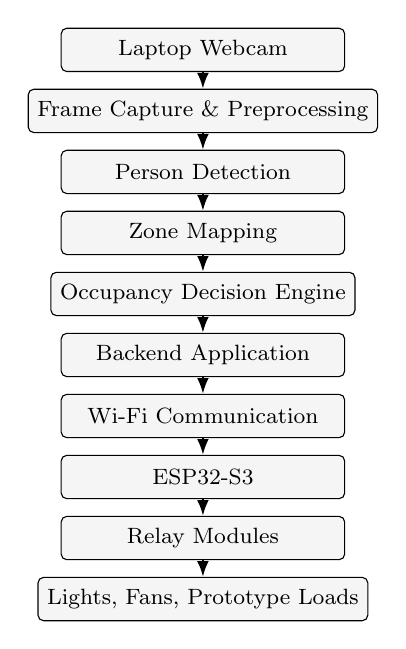
\begin{tikzpicture}[
    node distance=6pt,
    box/.style={rectangle, draw, rounded corners=2pt, minimum width=3.6cm, minimum height=0.55cm, align=center, font=\footnotesize, fill=gray!8},
    arr/.style={-{Latex[length=2mm]}, thick}
]
\node[box] (cam) {Laptop Webcam};
\node[box, below=of cam] (fp) {Frame Capture \& Preprocessing};
\node[box, below=of fp] (pd) {Person Detection};
\node[box, below=of pd] (zm) {Zone Mapping};
\node[box, below=of zm] (od) {Occupancy Decision Engine};
\node[box, below=of od] (be) {Backend Application};
\node[box, below=of be] (wifi) {Wi-Fi Communication};
\node[box, below=of wifi] (esp) {ESP32-S3};
\node[box, below=of esp] (relay) {Relay Modules};
\node[box, below=of relay] (load) {Lights, Fans, Prototype Loads};

\foreach \a/\b in {cam/fp, fp/pd, pd/zm, zm/od, od/be, be/wifi, wifi/esp, esp/relay, relay/load}
  \draw[arr] (\a) -- (\b);
\end{tikzpicture}
\caption{Data and control flow from camera input to physical switching.}
\label{fig:architecture}
\end{figure}

As shown in Fig.~\ref{fig:architecture}, the pipeline runs as follows: the laptop captures live video, detects people in each frame, estimates each person's floor position, and maps that position to a virtual zone. An occupancy decision engine then works out which appliances should be active based on current zone states, and a backend application forwards those decisions over Wi-Fi to the ESP32-S3. The ESP32-S3 does not perform any of the vision processing in this version of the system it receives already-decided commands and is responsible only for driving the relay channels connected to the room's loads, reporting its own state back, and keeping those relays in a safe condition on startup or after a dropped connection.

The system is organized into three layers:

\textit{Vision and AI layer} --- a laptop webcam feeding a Python and OpenCV pipeline, with a lightweight YOLO-based person-detection model handling frame preprocessing, zone assignment, and occupancy smoothing.

\textit{Backend and monitoring layer} --- a FastAPI backend responsible for real-time communication with the frontend, event logging, occupancy history, relay-state monitoring, energy estimation, and serving the web dashboard.

\textit{Embedded control layer} --- an ESP32-S3 handling Wi-Fi communication, relay switching, low-voltage prototype loads, a safe startup state, and command acknowledgement, with reconnection handling built in for when the network drops.

\section{Zone-Based Control and Occupancy Decision Logic}
The camera frame is divided into virtual zones representing distinct physical sections of the room. In the current prototype, three vertical zones are used, each tied to one relay channel, as summarized in Table~\ref{tab:zones}.

\begin{table}[htbp]
\caption{Zone-to-Relay Mapping (Current Prototype)}
\begin{center}
\begin{tabular}{|c|c|}
\hline
\textbf{Zone} & \textbf{Controlled Load} \\
\hline
Zone 1 & Relay 1 / Prototype appliance 1 \\
\hline
Zone 2 & Relay 2 / Prototype appliance 2 \\
\hline
Zone 3 & Relay 3 / Prototype appliance 3 \\
\hline
\end{tabular}
\label{tab:zones}
\end{center}
\end{table}

A detected person's zone is determined using the bottom centre point of their bounding box rather than its geometric centre, since the bottom-centre gives a closer estimate of where someone's feet are actually planted on the floor.

Switching appliances based on a single detection frame turns out to be a bad idea in practice: detection can momentarily fail because of motion blur, changes in lighting, partial occlusion, or plain model uncertainty, and reacting to every one of those blips would make the relays flicker constantly. To avoid that, Visualec applies timing and smoothing rules before any relay state actually changes:

\begin{itemize}
    \item An occupied zone switches its appliance ON after a short activation delay (on the order of one second).
    \item An empty zone switches its appliance OFF only after it has stayed empty for a longer deactivation delay, roughly ten to thirty seconds, so a person briefly stepping out doesn't trigger a shutdown.
    \item A single missed detection does not change anything the appliance holds its current state until the zone's status is confirmed over several frames.
    \item A person walking across a zone boundary is handled so as not to rapidly toggle the relays on either side.
    \item A manual override, when set by a user through the dashboard, is preserved temporarily rather than being immediately overwritten by automatic detection.
    \item An emergency mode exists that overrides automatic control entirely, for cases where every load needs to be forced off regardless of what the cameras are seeing.
\end{itemize}

\section{Energy Estimation}
Since the prototype does not yet include physical metering hardware, energy usage is estimated in software from each appliance's configured wattage and how long it has actually been active:
\begin{equation}
E \; \text{(kWh)} = \frac{P \, \text{(W)} \times t \, \text{(h)}}{1000}
\label{eq:energy}
\end{equation}
where $P$ is the appliance's rated power and $t$ is its runtime.

Two scenarios are compared using \eqref{eq:energy}. The \textit{baseline} consumption assumes every configured appliance stays on for the entire session, which approximates how a room behaves under manual or timer based control. The \textit{adaptive} consumption is calculated from each appliance's actual active runtime under zone-based control. The estimated savings follow directly:
\begin{equation}
E_{\text{saved}} = E_{\text{baseline}} - E_{\text{adaptive}}
\label{eq:savings}
\end{equation}
These figures are software estimates appropriate for the MVP stage and are not a substitute for physical measurement; later versions of the system are intended to validate them against smart meters or current-sensing modules.

\section{Current Prototype Scope}
The first working prototype is deliberately narrow in scope, built to prove out the full path from a camera frame to a switched relay rather than to cover every eventual use case. It currently includes one laptop webcam monitoring one room, divided into three virtual zones; person detection and zone-wise occupancy counting; three relay outputs driven by an ESP32-S3 over Wi-Fi; low-voltage prototype loads standing in for real lights and fans; and automatic control, a manual override, and a simulation mode, all visible through the dashboard alongside estimated energy analytics. The dashboard itself is meant to surface the live camera feed with detection boxes and zone boundaries drawn over it, per-zone occupancy counts, current relay and connectivity status, estimated power draw and savings, historical logs, emergency controls, and the configuration screens for zones and appliance mappings.

\section{Edge-AI Feasibility}
A natural next question is whether the vision pipeline could eventually run directly on the ESP32-S3 instead of a laptop, removing the laptop from the setup entirely. As it stands, that isn't practical: a standard YOLO model paired with a full OpenCV pipeline is far too heavy for the ESP32-S3's compute budget, and OpenCV itself is a software library rather than a trainable network, so there's nothing there to quantize --- only the detection model can be compressed that way. A genuinely edge-only version would need a much smaller, person-only detection architecture, INT8 quantization, a reduced input resolution, a camera wired directly into the ESP32-S3 rather than a laptop webcam, ESP-DL-compatible deployment, and simplified tracking logic; something like ESPDet-Pico is a plausible starting point for that architecture. For now, the laptop-based approach remains the main prototype, mostly because it gives better detection accuracy, a higher frame rate, easier debugging, and a setup that's simpler to demonstrate.

\section{Limitations}
The system's accuracy currently depends heavily on where the camera is mounted and how much of the room its field of view actually covers. Poor lighting reduces detection quality, and people who are partially hidden behind furniture or seated far from the camera are harder to detect reliably. A single camera is unlikely to cover a very large room on its own, and because AI processing still runs on a laptop rather than an embedded device, the system depends on that laptop staying connected and powered. The energy figures the dashboard reports are estimates rather than physical meter readings, and any move toward mains-voltage appliances would require certified wiring and electrical protection well beyond what the low-voltage prototype uses today. Deploying a camera-based system in real rooms also raises privacy questions that would need to be addressed directly before any wider rollout.

\section{Future Scope}
The architecture is built to extend rather than be replaced. Planned directions include supporting multiple cameras and ESP32-S3 nodes to cover larger or multiple rooms, integrating smart meters and current sensors to replace the current software estimates with real measurements, adding environmental sensors, moving analytics to the cloud, and building a mobile companion app. Longer-term ideas include occupancy heat maps, predictive energy optimization based on historical usage patterns, integration with classroom timetables and existing building-management systems, moving person detection onto edge hardware as discussed in Section VII, automated usage reports and recommendations, and eventual integration with renewable energy and battery-management systems as part of a broader smart-campus deployment.

\section{Conclusion}
Visualec is built around one fairly simple idea: energy should be spent where and when it's actually needed, not according to a fixed schedule or whatever a wall switch was left on. By combining a laptop camera, person detection, virtual zone mapping, an occupancy decision engine, and an ESP32-S3 driving relay hardware, the current prototype shows that zone-level control is achievable with hardware that's easy to get hold of and does not require rewiring a building. It is intentionally a first step the priority for this stage was proving that the whole pipeline, from a camera frame to a physical switch, works reliably end to end. What comes after is scaling that same idea across more zones, more rooms, and eventually a full building, with real metering replacing today's estimates along the way.

\begin{thebibliography}{00}
\bibitem{ref1} [Author(s)], ``[Title of a reference on occupancy-based lighting or HVAC control],'' [Conference/Journal], [Year].
\bibitem{ref2} [Author(s)], ``[Title of a reference on real-time person detection, e.g., YOLO-family models],'' [Conference/Journal], [Year].
\bibitem{ref3} [Author(s)], ``[Title of a reference on ESP32/microcontroller-based IoT relay control],'' [Conference/Journal], [Year].
\bibitem{ref4} [Author(s)], ``[Title of a reference on PIR sensors or occupancy-sensing limitations],'' [Conference/Journal], [Year].
\end{thebibliography}
% NOTE TO AUTHOR: References [1]-[4] above are placeholders. Replace each with an actual source you have read before submission.

\end{document}
